\section{20.11.23 : Rezolwenta}

\subsection{Definicje: rezolwenta projektywna i injektywna}

\begin{definition}[rezolwenta projektywna]
  Niech $A\in\ob \mathbf{A}$ będzie obiektem w kategorii abelowej. Wtedy kompleks $P^* \in Kom(\mathbf{A})$ razem z morfizmem $\epsilon:P^*\to\mathbf{A}$ nazywamy \buff{rezolwentą projektywną}, jeśli
  \begin{enumerate}
    \item $P^i$ są projektywne 
    \item $P^i=0$ dla $i>0$ 
    \item ciąg 
      $$...\to P^{-2}\to P^{-1}\to P^0\xrightarrow{\epsilon} A\to 0\to ...$$
      jest dokładny
  \end{enumerate}
\end{definition}

Ostatni warunek w powyższej definicji można również sformułować przy pomocy qis kompleksów:
\begin{center}\begin{tikzcd}
  ... \arrow[r] & P^{-2} \arrow[r]\arrow[d] & P^{-1} \arrow[r]\arrow[d] & P^0\arrow[d, "\epsilon"] \arrow[r] & 0 \arrow[r]\arrow[d] & ... \\ 
  ... \arrow[r] & 0 \arrow[r]      & 0 \arrow[r]      & A \arrow[r]                        & 0 \arrow[r] & ... 
\end{tikzcd}\end{center}

Zmienimy numerację obiektów kompleksu tak, że 
$$\color{blue}P_i:=P^{-i}$$

\begin{definition}[rezolwenta injektywna]
  Dla obiektu $A\in\ob\mathbf{A}$ jest definiowana w sposób analogiczny do rezolwenty injektywnej, tzn. jest kompleksem $I^*$ wraz z morfizmem $\iota : I^*\to A$ takim, że 
  \begin{enumerate}
    \item $I^i$ są injektywne 
    \item $I^i=0$ dla $i<0$ 
    \item ciąg 
      $$...\to 0\to A\xrightarrow{\iota} I^0\to I^1\to... $$
  \end{enumerate}
\end{definition}

\begin{example}
\item Ciąg dokładny $0\to \Z\to \Z\to \Z_2\to 0$, który pojawił się już w poprzednich przykładach, jest rezolwentą projektywną $\Z_2$:
  \begin{center}\begin{tikzcd}
    ...\arrow[r] & 0\arrow[r]\arrow[d] & \Z\arrow[r, "2\times"]\arrow[d] & \Z\arrow[r]\arrow[d] & 0\arrow[r]\arrow[d] & ...\\ 
    ...\arrow[r] & 0\arrow[r] & 0\arrow[r] & \Z_2\arrow[r] & 0\arrow[r] & ...
  \end{tikzcd}\end{center}
\item Dla pierścienia $\C$ traktowanego jako $\C[x]$-moduł mamy następującą rezolwentę
  \begin{center}\begin{tikzcd}
    ...\arrow[r] & 0 \arrow[r]\arrow[d] & \C[x] \arrow[r, "\cdot x"]\arrow[d] & \C[x] \arrow[r]\arrow[d, "x=0"] & 0\arrow[r]\arrow[d] & ... \\ 
    ...\arrow[r] & 0 \arrow[r] & 0\arrow[r] & \C \arrow[r] & 0 \arrow[r] & ...
  \end{tikzcd}\end{center}
\item Rezolwenta $\C$ jako $\C[x, y]$-modułu jest konstruowana w sposób analogiczny do tego wyżej:
  \begin{center}\begin{tikzcd}[column sep=small, row sep=small]
    ...\arrow[r] & \C[x, y]\arrow[r]& \C[x. y] \oplus \C[x, y]\arrow[r] & \C[x, y] \arrow[r, "\substack{x=0 \\ y=0}"] & \C \arrow[r] & 0 \arrow[r] & ... \\ 
                 & R\arrow[r, mapsto] & (yR) \oplus (xR)\\ 
                 & & q\oplus p\arrow[r, mapsto] & xq - yp
  \end{tikzcd}\end{center}
\end{example}

\subsection{Jednoznacnzość rezolwenty projektywnej} 

\begin{definition}[homotopia morfizmów]
  Niech $\mathbf{A}$ będzie kategorią abelową (addytywną). Morfizmy kompleksów $f, g:A^*\to B^*$ są \buff{homotopijne} ($f\sim g$), jeśli istnieje między nimi homotopia, tzn. ciąg odwzorowań $h^i:A^i\to B^{i-1}$ taki, że
  $$f^i-g^i=h^{i+1}\circ d_A^i+d_B^{i-1}\circ h^i$$
  \begin{center}
    \begin{tikzcd}[row sep=large, column sep=large]
    ...\arrow[r] & A^{i-1}\tikzmark{Ai-1} \arrow[r]\arrow[d, "g" left, xshift=-1mm]\arrow[d, "f" right, xshift=1mm] & A^i \tikzmark{Ai} \arrow[dl, "h^i" above, yshift=1mm, blue]\arrow[d, "g" left, xshift=-1mm]\arrow[d, "f" right, xshift=1mm]\arrow[r] \arrow[d, to path = {}] & A^{i+1} \tikzmark{Ai+1} \arrow[d, "g" left, xshift=-1mm] \arrow[d, "f" right, xshift=1mm] \arrow[dl, "h^{i+1}" below right, yshift=-1mm, blue] \arrow[r] & ... \\ 
    ...\arrow[r] & B^{i-1} \tikzmark{Bi-1} \arrow[r] & B^i \tikzmark{Bi} \arrow[r] & B^{i+1} \tikzmark{Bi+1} \arrow[r] & ...
  \end{tikzcd}
  \begin{tikzpicture}[remember picture, overlay]
    \draw[orange, ->, rounded corners] ([xshift=-1mm]pic cs:Ai) to ([xshift=1mm, yshift=3mm]pic cs:Bi-1) to ([xshift=-3mm, yshift=3mm]pic cs:Bi);
    \draw[orange, ->, rounded corners] ([xshift=1mm, yshift=-1mm]pic cs:Ai) to ([xshift=-6mm, yshift=-1mm]pic cs:Ai+1) to ([xshift=2mm, yshift=4mm]pic cs:Bi);
  \end{tikzpicture}
\end{center}
\end{definition}

\begin{example}
\item W przypadku przestrzeni topologicznych o homotopii dwóch funkcji $f, g:X\to Y$ można myśleć jako o funkcji $H$ z cylindra $X\times I$ w przestrzeń $Y$:
  \begin{center}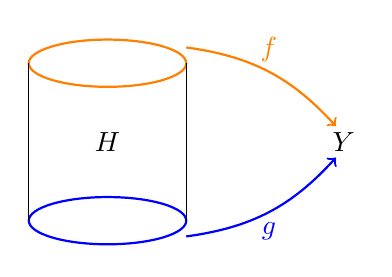
\begin{tikzpicture}
    \draw[blue, thick] (0, 0) ellipse(1 and 0.3);
    \draw[orange, thick] (0, 2) ellipse(1 and 0.3);

    \draw (-1, 0)--(-1, 2);
    \draw (1, 0)--(1, 2);

    \node at (3, 1) {$Y$};

    \path[->] (1, -0.2) edge [bend right=20, thick, blue] node [midway, below] {$g$} (2.9, 0.8);
    \path[->] (1, 2.2) edge [bend left=20, orange, thick] node [midway, above] {$f$} (2.9, 1.2);

    \node at (0, 1) {$H$};
  \end{tikzpicture}\end{center}

  Możemy do tego przyłożyć wiedzę o kompleksach, jeśli pod $X$ kryją się sympleksy. Wtedy mamy
  \begin{center}\begin{tikzpicture}[scale=1.5]
    \draw (0, 0) ellipse(1 and 0.3);
    \draw (0, 2) ellipse(1 and 0.3);

    \draw (-1, 0)--(-1, 2);
    \draw (1, 0)--(1, 2);

   % \draw[dashed] (-0.6, -0.1)--(-0.2, -0.15)--(-0.4, 0.1)--cycle;
   % \draw[dashed] (-0.4, 0.1)--(0, 0.15)--(-0.2, -0.15)--cycle;
   % \draw[dashed] (-0.2, -0.15)--(0.2, -0.15)--(0, 0.15)--cycle;
   % \draw[dashed] (0.2, -0.15)--(0.4 ,0.1)--(0, 0.15)--cycle;
   % \draw[dashed] (0.2, -0.15)--(0.4, 0.1)--(0.6, -0.1)--cycle;

    \draw[dashed] (-0.6, -0.1)--(-0.4, 0.1)--(-0.2, -0.15)--(0, 0.15)--(0.2, -0.15)--(0.4, 0.1)--(0.6, -0.1);
    \draw[dashed] (-0.4, 0.1)--(0, 0.15)--(0.4, 0.1);
    \draw (-0.6, -0.1)--(-0.2, -0.15)--(0.2, -0.15)--(0.6, -0.1);

    \draw (-0.6, 1.9)--(-0.2, 1.85)--(-0.4, 2.1)--cycle;
    \draw (-0.4, 2.1)--(0, 2.15)--(-0.2, 1.85)--cycle;
    \draw (-0.2, 1.85)--(0.2, 1.85)--(0, 2.15)--cycle;
    \draw (0.2, 1.85)--(0.4, 2.1)--(0, 2.15)--cycle;
    \draw(0.2, 1.85)--(0.4, 2.1)--(0.6, 1.9)--cycle;

    \draw(-0.6, -0.1)--(-0.6, 1.9);
    \draw(-0.2, -0.15)--(-0.2, 1.85);
    \draw(0.2, -0.15)--(0.2, 1.85);
    \draw(0.6, -0.1)--(0.6, 1.9);

    \draw[dashed] (-0.4, 0.1)--(-0.4, 2.1);
    \draw[dashed] (0, 0.1)--(0, 2.1);
    \draw[dashed] (0.4, 0.1)--(0.4, 2.1);

    \draw (2, 1.8)--(3, 2.2)--(1.8, 2.2)--cycle;
    \draw (2, -0.2)--(3, 0.2);
    \draw (2, -0.2)--(1.8, 0.2);
    \draw[dashed] (3, 0.2)--(1.8, 0.2);

    \draw (1.8, 0.2)--(1.8, 2.2);
    \draw (3, 0.2)--(3, 2.2);
    \draw (2, -0.2)--(2, 1.8);

    \node (HD) at (4, 1.5) {$H(\Delta)$};

    \path[->] (HD) edge [bend left=20] (2.4, 1);

    \node at (2.2, 2.1) {$\Delta$};
    \node at (2.5, -0.2) {$\partial$};

    \node at (4, 0.6) {$\substack{\partial H(\Delta)=f(\Delta)-g(\Delta)+\\+H(\partial\Delta)}$};
  \end{tikzpicture}\end{center}
\end{example}

\begin{fact}$ $

  \begin{enumerate}[label=(\alph*)]
    \item Relacja homotopijnej równoważności $\sim$ odwzorowań między ustalonymi kompleksami $A^*, B^*$ jest relacją równoważności
    \item Morfizmy $\sim 0$ tworzą "ideał", to znaczy 
      $$g, f\sim 0\implies f+g\sim 0$$
      $$(\forall\;k:B^*\to C^*,\; l:C^*\to A^*)\;f\sim 0\implies kf, fl\sim 0$$
    \item $f\sim g\implies H^i(f)=H^i(g)$
    \item Jeśli \begin{tikzcd}A^*\arrow[r, yshift=1mm, "f" above] & B^*\arrow[l, yshift=-1mm, "g" below]\end{tikzcd} są takie, że $fg\sim id_B$ oraz $gf\sim id_A$, to $f,g$ są qis oraz $H^i(f)=H^i(g)^{-1}$.
  \end{enumerate}
\end{fact}

\begin{proof}
  \begin{enumerate}[label=(\alph*)]
    \item Niech $f\overset{h}{\sim} g\overset{h'}{\sim} l$, wówczas $f\overset{h+h'}{\sim}l$. Wiemy więc, że 
      $$\begin{matrix}
        f-g = dh+hd\\ 
        g-l=dh'+h'd
      \end{matrix}$$
      dodając oba równania stronami, dostajemy
      $$f-l=(f-g)+(g-l)=(dh+hd)+(dh'+h'd)=(dh+dh')+(hd+h'd)=d(h+h')+(h+h')d.$$
    \item Jeśli $f, g\sim 0$ tak, że $f-0=dh+hd$ oraz $g-0=dh'+h'd$. Wtedy
      $$f+g=(f-0)+(g-0)=(dh+hd)+(dh'+h'd)=d(h+h')+(h+h')d.$$

      Pokażemy teraz, że dla $f\sim 0$ oraz dla dowolnego $k:B^*\to C^*$ mamy $kf\sim 0$. Rysując diagram
      \begin{center}
        \begin{tikzcd}[column sep=large, row sep=large, /tikz/column 1/.style={column sep=1mm}]
        A^*: & \bullet \arrow[d, "f" left] \arrow[r, dashed] & \bullet \tikzmark{A2} \arrow[d, "f" left] \arrow[r, dashed] \arrow[dl, "h" above] & \bullet \arrow[d, "f" left] \arrow[r, dashed] \arrow[dl, "h" above] & \bullet \arrow[d, "f" left] \\ 
        B^*: & \bullet \tikzmark{B1} \arrow[r, dashed] \arrow[d, "k" left] & \bullet \arrow[r, dashed, blue] \arrow[d, "k" left, red] & \bullet \arrow[r, dashed] \arrow[d, "k" left, blue] & \bullet \arrow[d, "k" left] \\ 
        C^*: & \bullet \tikzmark{C1} \arrow[r, dashed] & \bullet \arrow[r, dashed, red] & \bullet \arrow[r, dashed] & \bullet
        \end{tikzcd}
        \begin{tikzpicture}[remember picture, overlay]
          \draw[orange, ->, rounded corners] ([xshift=-2mm, yshift=-2mm]pic cs:A2) to ([xshift=2mm, yshift=2mm]pic cs:B1) node [right] {$k\circ h$} to ([xshift=2mm, yshift=2mm]pic cs:C1);
        \end{tikzpicture}
      \end{center} 
      Wiemy, że $f^i=h^{i+1}d+dh^i$, a dalej
      $$k^if^i=k^i(h^{i+1}d+dh^i)=k^i(h^{i+1}d)+k^i(dh^i)=(k^ih^{i+1})d+({\color{red}k^{i}d})h^i=(k^ih^{i})d+{\color{blue}d(k^{i-1}}h^{i})$$

    \item Wystarczy sprawdzić, że $f\sim 0\implies H^i(f)=0$. Niech $[a]\in H^i(f)$ zadaje klasę kohomologii, czyli $a\mapsto 0$ przez różniczkę $A^i\to A^{i+1}$.
      \begin{center}
        \begin{tikzcd}[/tikz/row 1/.style={row sep=1mm}, /tikz/row 3/.style={row sep=1mm}]
          & a\arrow[d, phantom, sloped, "\in"] \arrow[r, mapsto] & 0 \\ 
          A^{i-1} \arrow[r] \arrow[d] & A^i \arrow[r] \arrow[d] \arrow[dl, "h^i" above, blue] & A^{i+1} \arrow[d] \arrow[dl, "h^{i+1}" above, blue] \\ 
          B^{i-1} \arrow[r] & B^i \arrow[r] & B^{i+1} \\ 
          ? \arrow[r, dashed] & f^i(a)\arrow[r, mapsto] \arrow[u, phantom, sloped, "\in"] & 0
        \end{tikzcd}
      \end{center}
      Wiemy, że 
      $$f^i(a)=h^{i+1}\underbrace{d(a)}_{=0}+dh^i(a)=dh^i(a)$$
      czyli $h^i(a)$ jest w ramach $?$.
    \item Wynika z warunku c).
  \end{enumerate}
\end{proof}

\begin{fact}
  Niech $P^*\to X$ oraz $Q^*\to Y$ będą rezolwentami projektywnymi, a $f:X\to Y$ będzie morfizmem.
  \begin{enumerate}
    \item Istnieje morfizm rezolwent $R(f):P^*\to Q^*$ rozszerzający $f$ w sensie komutowania driagramu
      \begin{center}\begin{tikzcd}
        ... \arrow[r] & P^0\arrow[r, "\epsilon_x"]\arrow[d, "R(f)^0"] & X \arrow[d, "f"] \\ 
        ... \arrow[r] & Q^0 \arrow[r, "\epsilon_y"] & Y
      \end{tikzcd}\end{center}
      oraz diagramów "dalej na lewo".
    \item $R(f)$ jak wyżej jest jedyny z dokładnością do homotopii.
  \end{enumerate}
\end{fact}

\begin{conclusion}
  Gdy $Y=X$ i $f=id_X$, to mamy jedyne z dokładnością do homotopii przekształcenie między dwoma różnymi rezolwentami $X$.

  \begin{center}\begin{tikzcd}
    P^*\arrow[r]\arrow[d, "R" right, bend left=20] & X\arrow[d, "id"]\\ 
    Q^*\arrow[r]\arrow[u, bend left=20, "L" lef] & X
  \end{tikzcd}\end{center}
\end{conclusion}

\begin{proof}
  \begin{enumerate}[label=(\alph*)]
    \item Konstruujemy ten morfizm 
      \begin{center}\begin{tikzcd}
        P_0\arrow[r, "\epsilon_X"]\arrow[d, dashed] \arrow[dr, rounded corners, to path={([yshift=-4mm]\tikztostart) -| ([xshift=-5mm]\tikztotarget)}, blue] & X\arrow[r]\arrow[d, "f" right] & 0 \\ 
        Q_0\arrow[r, "\epsilon_Y" below] & Y \arrow[r] & 0
      \end{tikzcd}\end{center}
      Strzałka $P_0\to Q_0$ istnieje, ponieważ $P_0$ jest modułem projektywny, i $Q_0\to Y$ jest surjekcją. Czyli mamy diagram
      \begin{center}\begin{tikzcd}
        P_0\arrow[d, dashed]\arrow[dr] \\ 
        Q_0\arrow[r] & Y \arrow[r] & 0
      \end{tikzcd}\end{center}
  \end{enumerate}

  {\large\color{red}CHYBA WRÓCIĆ}
\end{proof}
